\chapter{Diseño y Desarrollo}
\label{ch:modelo}

Este capítulo describirá el diseño y desarrollo del modelo de predicción de demanda y optimización de ingresos. El primer paso será presentar los \emph{data sets} utilizados. El segundo paso consistirá en describir el modelo, sus módulos, el funcionamiento y la arquitectura.

\section*{Data Sets}
Para la construcción del modelo de predicción de demanda se utilizaron tres data sets que contienen la información suficiente para poder hacer un pronóstico efectivo de la demanda de una propiedad.

\subsection*{Detalle de reservaciones}


El primer data set utilizado fue extraído directamente del sistema de gestión de propiedades (PMS) y contiene información detallada de todas las reservaciones generadas en la propiedad, así como la información de las estancias pasadas. Para poder obtener esta información se realizarón procesos automáticos de extracción, transformación y carga de información. 

A continuación se presenta el detalle de la información obtenida del PMS así como el diccionario de datos y un breve resumen de la información en cada una de las columnas.

\subsubsection*{Diccionario de Datos}


\begin{itemize}
  \item rsrv\_code: Código de confirmación de la reservación
  \item date\_create: Fecha y hora de creación de la reserva
  \item date\_in: Fecha de llegada a la propiedad
  \item date\_out: Fecha de salida de la propiedad
  \item nights: Número de noches de la reservación en el hotel
  \item prop\_code: Código de la propiedad dentro del sistema de gestión de propiedades
  \item mkt\_sgm: Segmento de mercado del huésped amparado en la reservación
  \item Dia\_Sem: Día de la semana de la fecha de llegada del huésped
  \item rate\_code: Código de tarifa
  \item bucket: Categoría de tarifa
  \item Ingresos: Ingresos obtenidos por la renta habitación de la reservación
  \item rsrv\_src: Canal de generación de la reservación
  \item rsrv\_type: Tipo de reservación
  \item room\_type: Tipo de habitación
  \item PAX: Número de personas amparadas por la reservación
\end{itemize}

\subsubsection*{Resumen de datos}

\begin{table}[H]
\begin{tabular}{lllll}
Variable     & Tipo de dato & Min        & Max        & Media \\
rsrv\_code   & Big Int      & 6265739    & 9053354    & NA    \\
date\_create & Fecha        & 2016-07.20 & 2018-01-01 & NA    \\
date\_ in    & Fecha        & 2017-01-01 & 2017-12-31 & NA    \\
date\_out    & Fecha        & 2017-01-02 & 2018-01-01 & NA    \\
prop\_code   & Factor       & NA         & NA         & NA    \\
mkt\_sgm     & Factor       & NA         & NA         & NA    \\
Dia\_sem     & Factor       & NA         & NA         & NA    \\
rate\_code   & Factor       & NA         & NA         & NA    \\
bucket       & Factor       & NA         & NA         & NA    \\
rsrv\_src    & Factor       & NA         & NA         & NA    \\
rsrv\_type   & Factor       & NA         & NA         & NA    \\
Ingresos     & Float        & 0          & 3900       & 1449  \\
PAX          & Integer      & 0          & 5          & 1.271 \\
\end{tabular}
\caption{Resumen de datos obtenidos del PMS} 
\end{table}

Es importante resaltar que los datos fueron trabajados para presentarse de manera desagregada, es decir, si una reservación ampara una estancia de 5 noches, en el \emph{data set final} se presenta un registro por cada noche de la estancia, por ejemplo:

\begin{knitrout}
\definecolor{shadecolor}{rgb}{0.969, 0.969, 0.969}\color{fgcolor}\begin{table}[H]
\centering\rowcolors{2}{gray!6}{white}

\begin{tabular}{r|l|l|l|r|l}
\hiderowcolors
\hline
rsrv\_code & date\_create & date\_in & date\_out & nights & room\_type\\
\hline
\showrowcolors
6265739 & 2016-07-20 18:31:59 & 2017-04-07 & 2017-04-08 & 1 & NSK\\
\hline
6265739 & 2016-07-20 18:31:59 & 2017-04-08 & 2017-04-09 & 1 & NSK\\
\hline
6265739 & 2016-07-20 18:31:59 & 2017-04-09 & 2017-04-10 & 1 & NSK\\
\hline
6265739 & 2016-07-20 18:31:59 & 2017-04-10 & 2017-04-11 & 1 & NSK\\
\hline
6265739 & 2016-07-20 18:31:59 & 2017-04-11 & 2017-04-12 & 1 & NSK\\
\hline
6265739 & 2016-07-20 18:31:59 & 2017-04-12 & 2017-04-13 & 1 & NSK\\
\hline
\end{tabular}
\caption{DataSet detalle de reservas} 
\rowcolors{2}{white}{white}
\end{table}
\end{knitrout}

Como se puede observar, el número de reservación es el mismo en los seis registros, lo mismo ocurre con la fecha de creación, las noches y el tipo de habitación, sin embargo, la fecha de entrada y la fecha de salida va cambiando en cada registro, lo que nos permite medir la demanda generada por aquellas reservaciones que contemplan más de una noche de estancia en la propiedad. 

\subsubsection*{Curvas de Pickup}

Del data set anterior podemos obtener las curvas de pickup del hotel. Estas curvas describen el comportamiento de las reservaciones para la propiedad en cuestión ya que mediante ellas podemos saber con cuanto tiempo de anticipación se comienzan a reservar las habitaciones de la propiedad. A continuación se muestran las curvas de pickup para esta propiedad:

\begin{figure}[H]
  \centering
      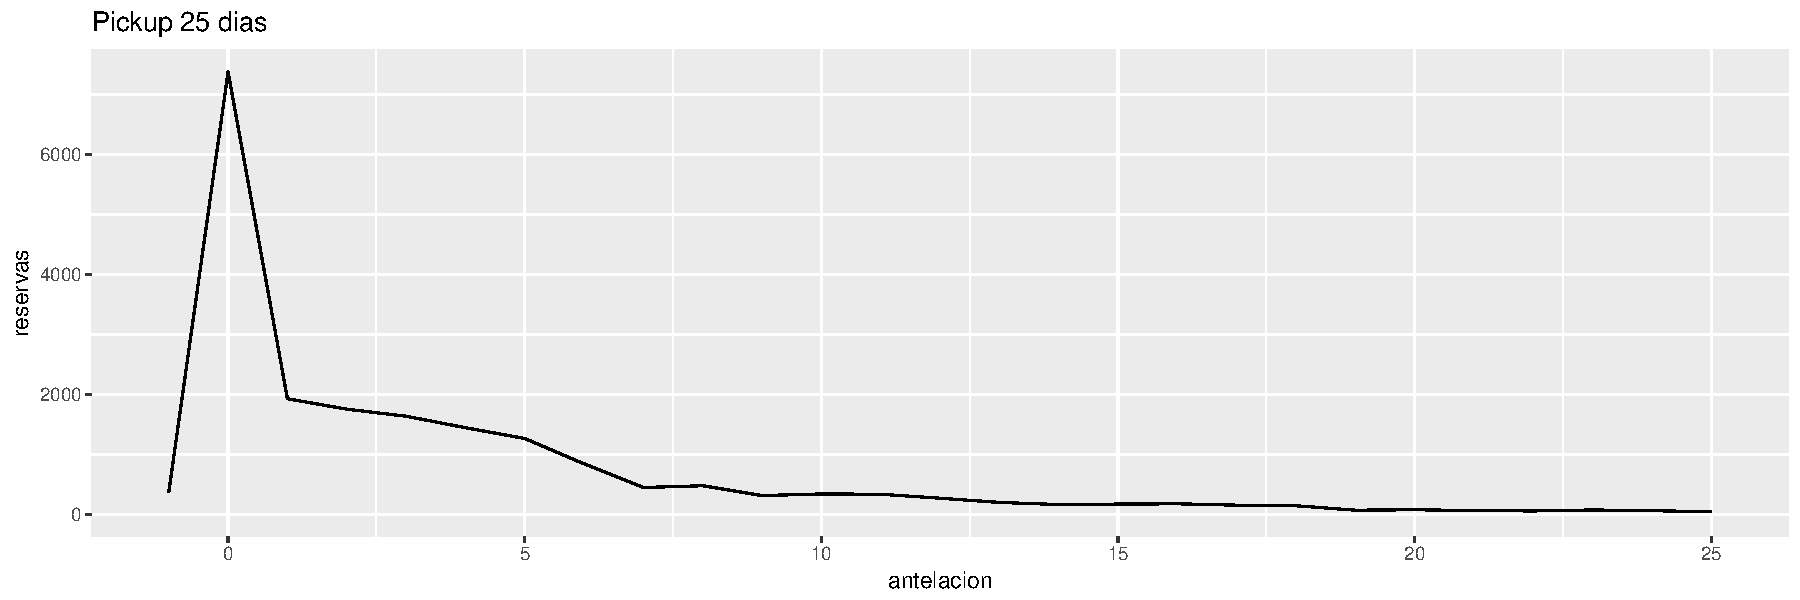
\includegraphics[width=\maxwidth,height=10cm]{figures/pickupzoom-1}  
  \caption{Curva de pickup}
\end{figure}

Analizando las gráficas presentadas anteriormente podemos concluír que la demanda de esta propiedad comienza 25 días antes de la llegada del huésped al hotel, e incrementa considerablemente 5 días antes de la llegada del huésped al hotel. Este dato nos indica que el huésped comienza a buscar una habitación dentro de esta propiedad en un lapso no mayor a 25 días antes de emprender su viaje y la demanda de habitaciones incrementa considerablemente 5 días antes de la fecha de llegada a la propiedad.

Las curvas de \emph{pickup} son importantes dentro del proceso de toma de decisiones ya que le indican al equipo que gestiona la propiedad el tiempo de antelación con el cual deberían llevar a cabo las acciones necesarias para poder optimizar el ingreso generado por la renta de habitaciones.

\subsection*{Ocupación de la propiedad}

El segundo \emph{data set} con el que se trabajó contiene las líneas de tiempo de los níveles de ocupación de la propiedad. Este set de datos es de suma importancia ya que proporciona información relevante con respecto a las temporalidades del hotel, mismas que deben ser reflejadas en el resultado del modelo.

Las temporalidades del hotel pueden ser desde periodos con alta o baja ocupación, inclusive por día de la semana ya que al ser un hotel enfocado a viajeros de negocio, se esperaría tener una alta ocupación los días laborales (Lunes a Jueves) y una baja ocupación los fines de semana (Viernes a Domingo).

A continuación se presenta el contenido de este \emph{data set}:

\begin{figure}[H]
  \centering
      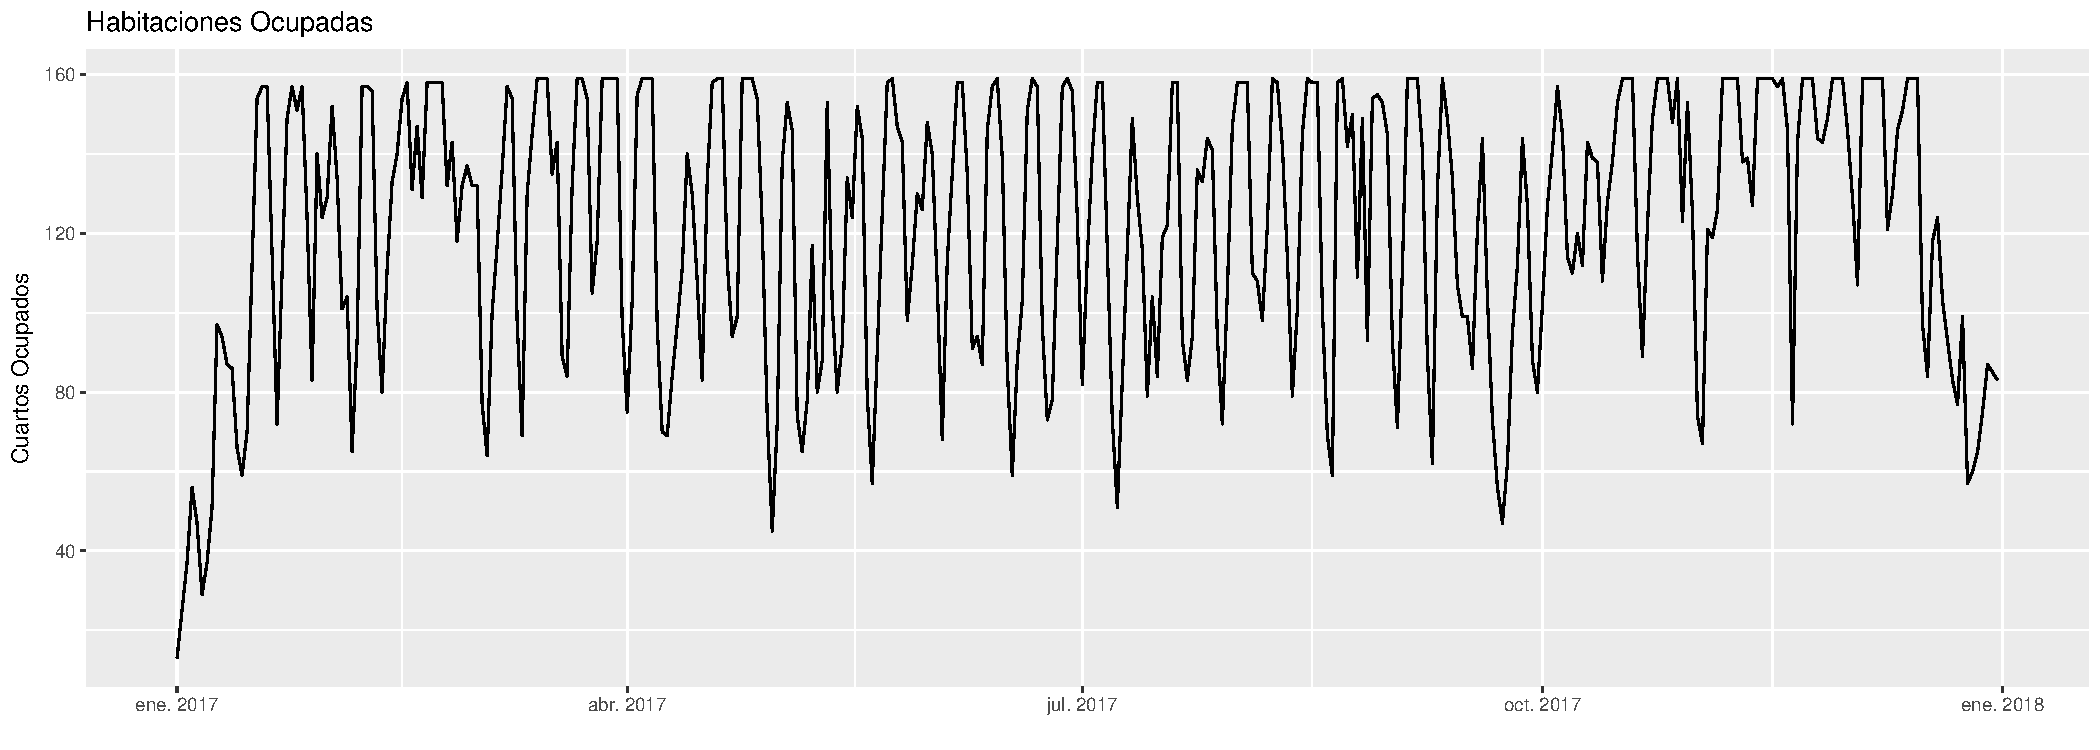
\includegraphics[width=\maxwidth,height=10cm]{figures/HabitacionesOcupadas-1}   
  \caption{\% Ocupación 2017}
\end{figure}


Como se puede observar en la gráfica presentada anteriormente, esta propiedad tiene altos níveles de ocupación (alredor del 75\% de ocupación) agotando en repetidas ocasiones su inventario disponible (159 cuartos). Las caídas en los níveles de ocupación ocurren los fines de semana, lo cual confirma que el mercado objetivo de la propiedad estudiada es el turismo de negocios.

A continuación se presenta una gráfica de níveles de ocupación por día de la semana:

\begin{figure}[H]
  \centering
      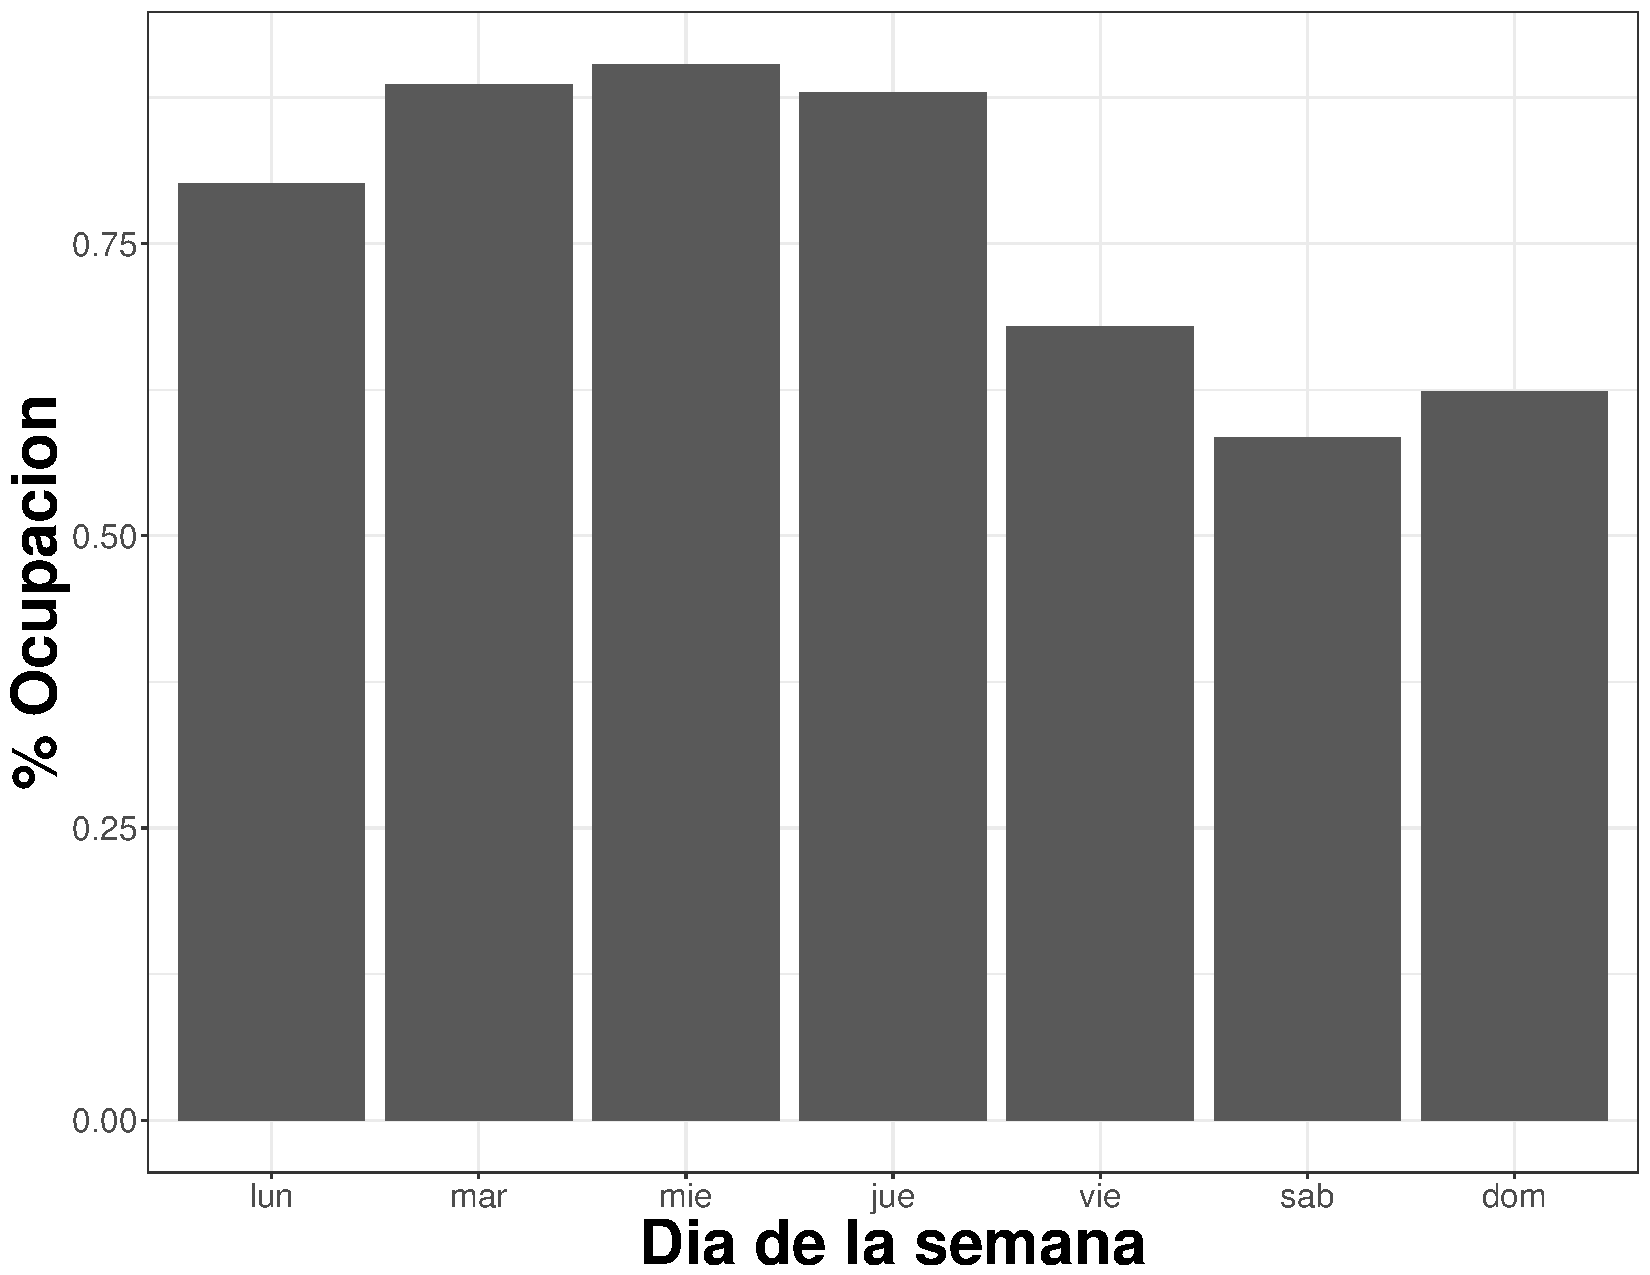
\includegraphics[width=\maxwidth,height=10cm]{Figures/Ocupacion_Dia_Semana-1}   
  \caption{Ocupación por día de la semana}
\end{figure}



\subsection*{Tarifa Promedio de la propiedad}

El tercer conjunto de datos utilizado contiene los valores de la tarifa promedio \emph{ADR: Average Daily Rate} en el tiempo. Estos datos fueron obtenidos directamente del PMS y es el resultado de sumar los ingresos generados por las habitaciones divididos por el número total de cuartos vendidos. 

A continuación se presenta la línea de tiempo con los valores para la tarifa promedio a lo largo del tiempo.

\begin{figure}[H]
  \centering
      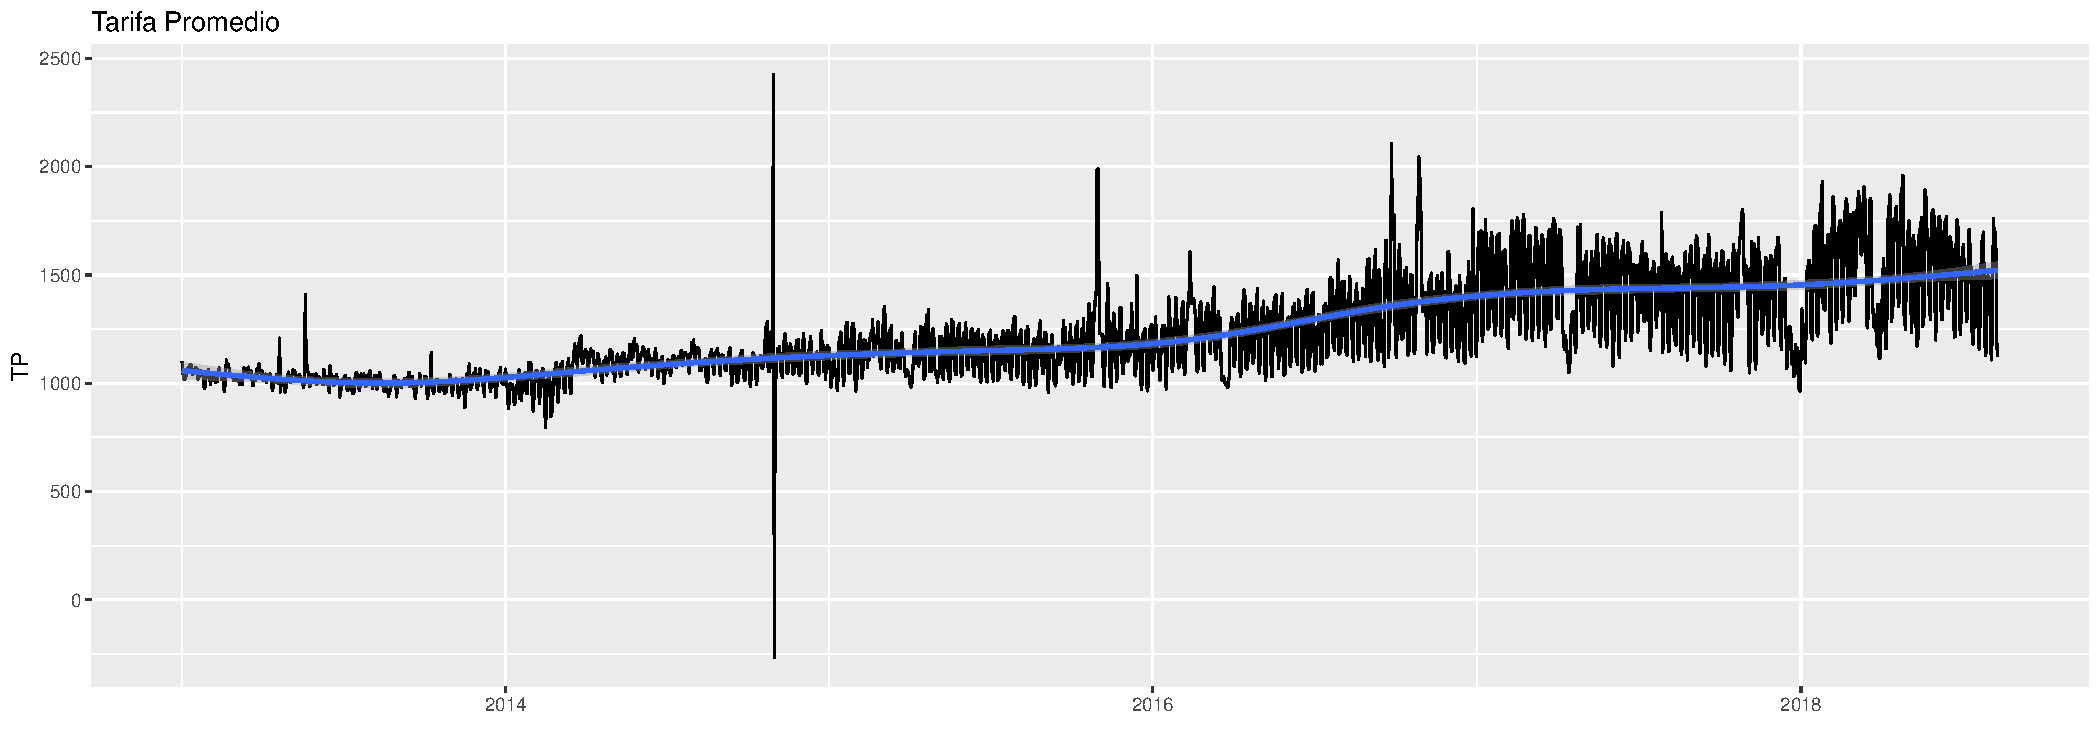
\includegraphics[width=\maxwidth,height=10cm]{figures/IndicadoresTarifaPromedio-1}    
  \caption{Tarifa Promedio 2017}
\end{figure}


De esta última gráfica se puede observar que los precios siguen una tendencia positiva con respecto al tiempo, a medida que pasa el tiempo, los precios incrementan, sin embargo podemos notar también que a medida que pasa el tiempo los precios varían más. Si contrastamos la información presentada en la gráfica de la tarifa promedo vs el tiempo (Figura 4.4) y la presentada en la gráfica de ocupación vs el tiempo (Figura 4.2) podemos ver que aunque los precios han aumentado en esta propiedad, las tendencias en los níveles de ocupación permanecen constantes.

\subsection*{Precios Públicos en el tiempo}

Como se mencionó anteriormente, una propiedad típicamente tiene diferentes precios disponibles para cada uno de los segmentos de mercado a los que atiende. La tarifa que se ofrece al público que llega al hotel sin una reservación previa se le conoce como \emph{tarifa pública} y generalmente es la tarifa con el precio mas alto de la cúal desprenden todas las demás tarifas, es decir, el conjunto de tarifas disponible en el hotel serán descuentos realizados sobre la \emph{tarifa pública}.

El tercer data set utilizado durante el desarrollo del modelo, contiene la información de las tarifas públicas de la propiedad y su competencia a lo largo del tiempo. Esto nos ayudará a conocer el precio del producto ofrecido en el mercado objetivo, de tal forma que los precios arrojados por el modelo se encuentren siempre dentro del mercado.

Los precios de la competencia fueron obtenidos de las páginas electrónicas de las agencias en línea, booking.com y expedia.com principalmente.

A continuación se presentan las líneas de tiempo con los precios públicos para el conjunto de propiedades.

\begin{figure}[H]
  \centering
      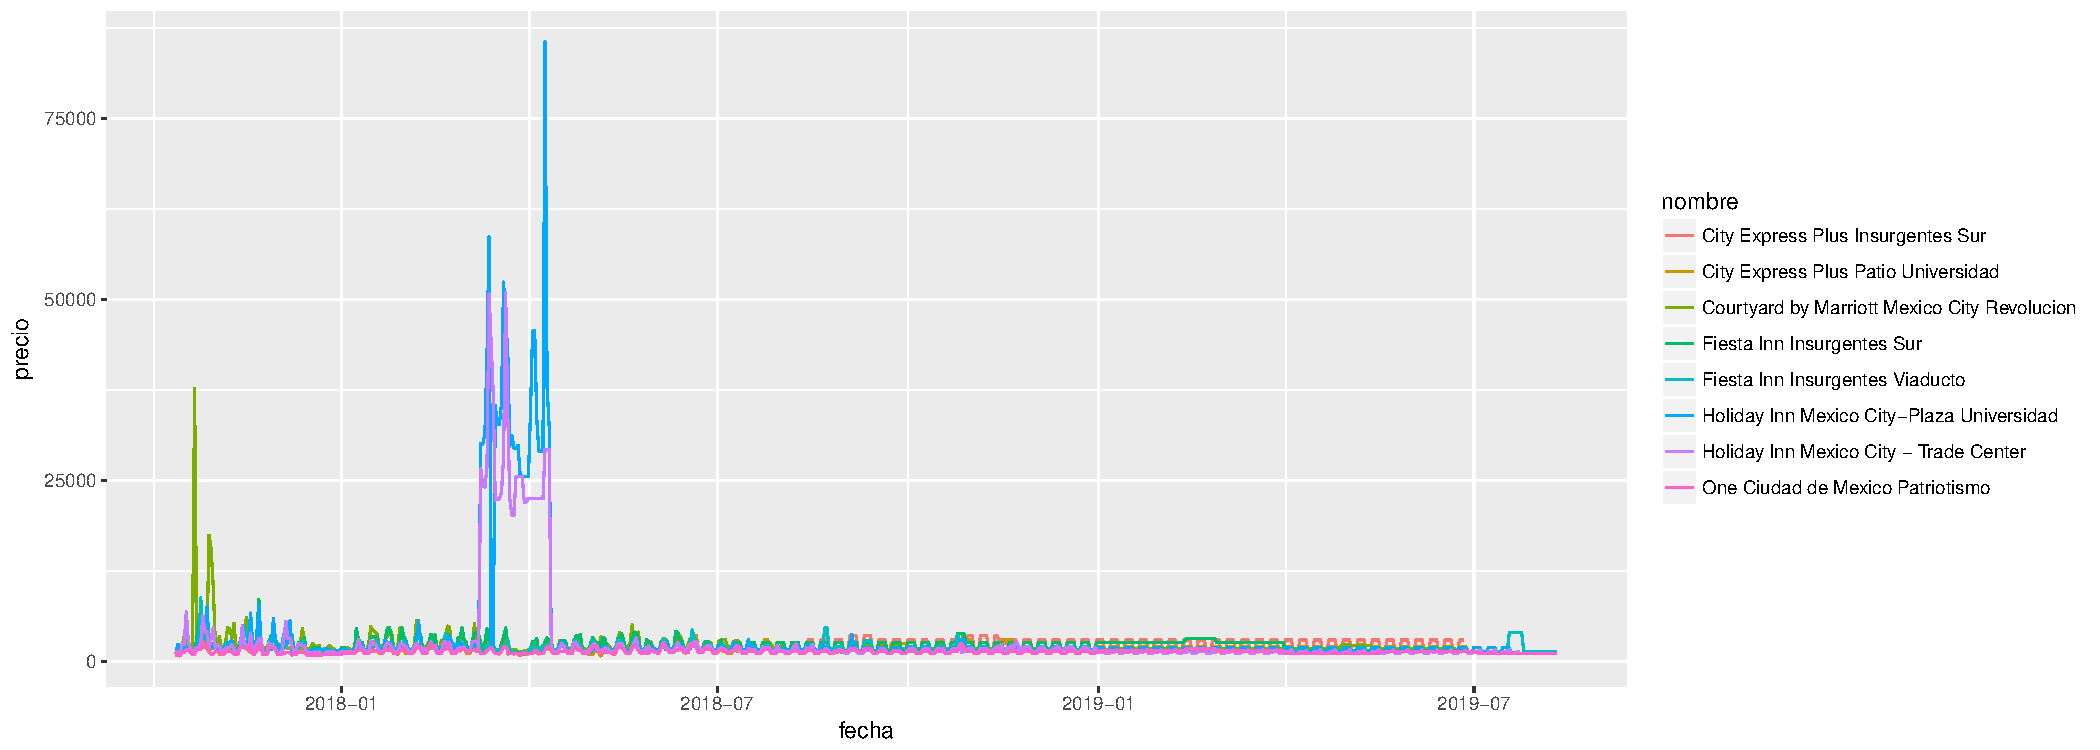
\includegraphics[width=\maxwidth,height=8cm]{figures/PreciosGraf-1}    
  \caption{Precios de la competencia en el tiempo}
\end{figure}


En la gráfica anterior se puede observar que hay algunos datos atípicos ya que es poco probable encontrar habitaciones en este segmento de hoteles por arriba de los \$4,000 MXN. Para confirmar esto se realizó una gráfica de caja y bigotes (boxplot) en la cuál se puede observar a primera vista los datos atípicos contenidos en el \emph{data set}.

\begin{figure}[H]
  \centering
      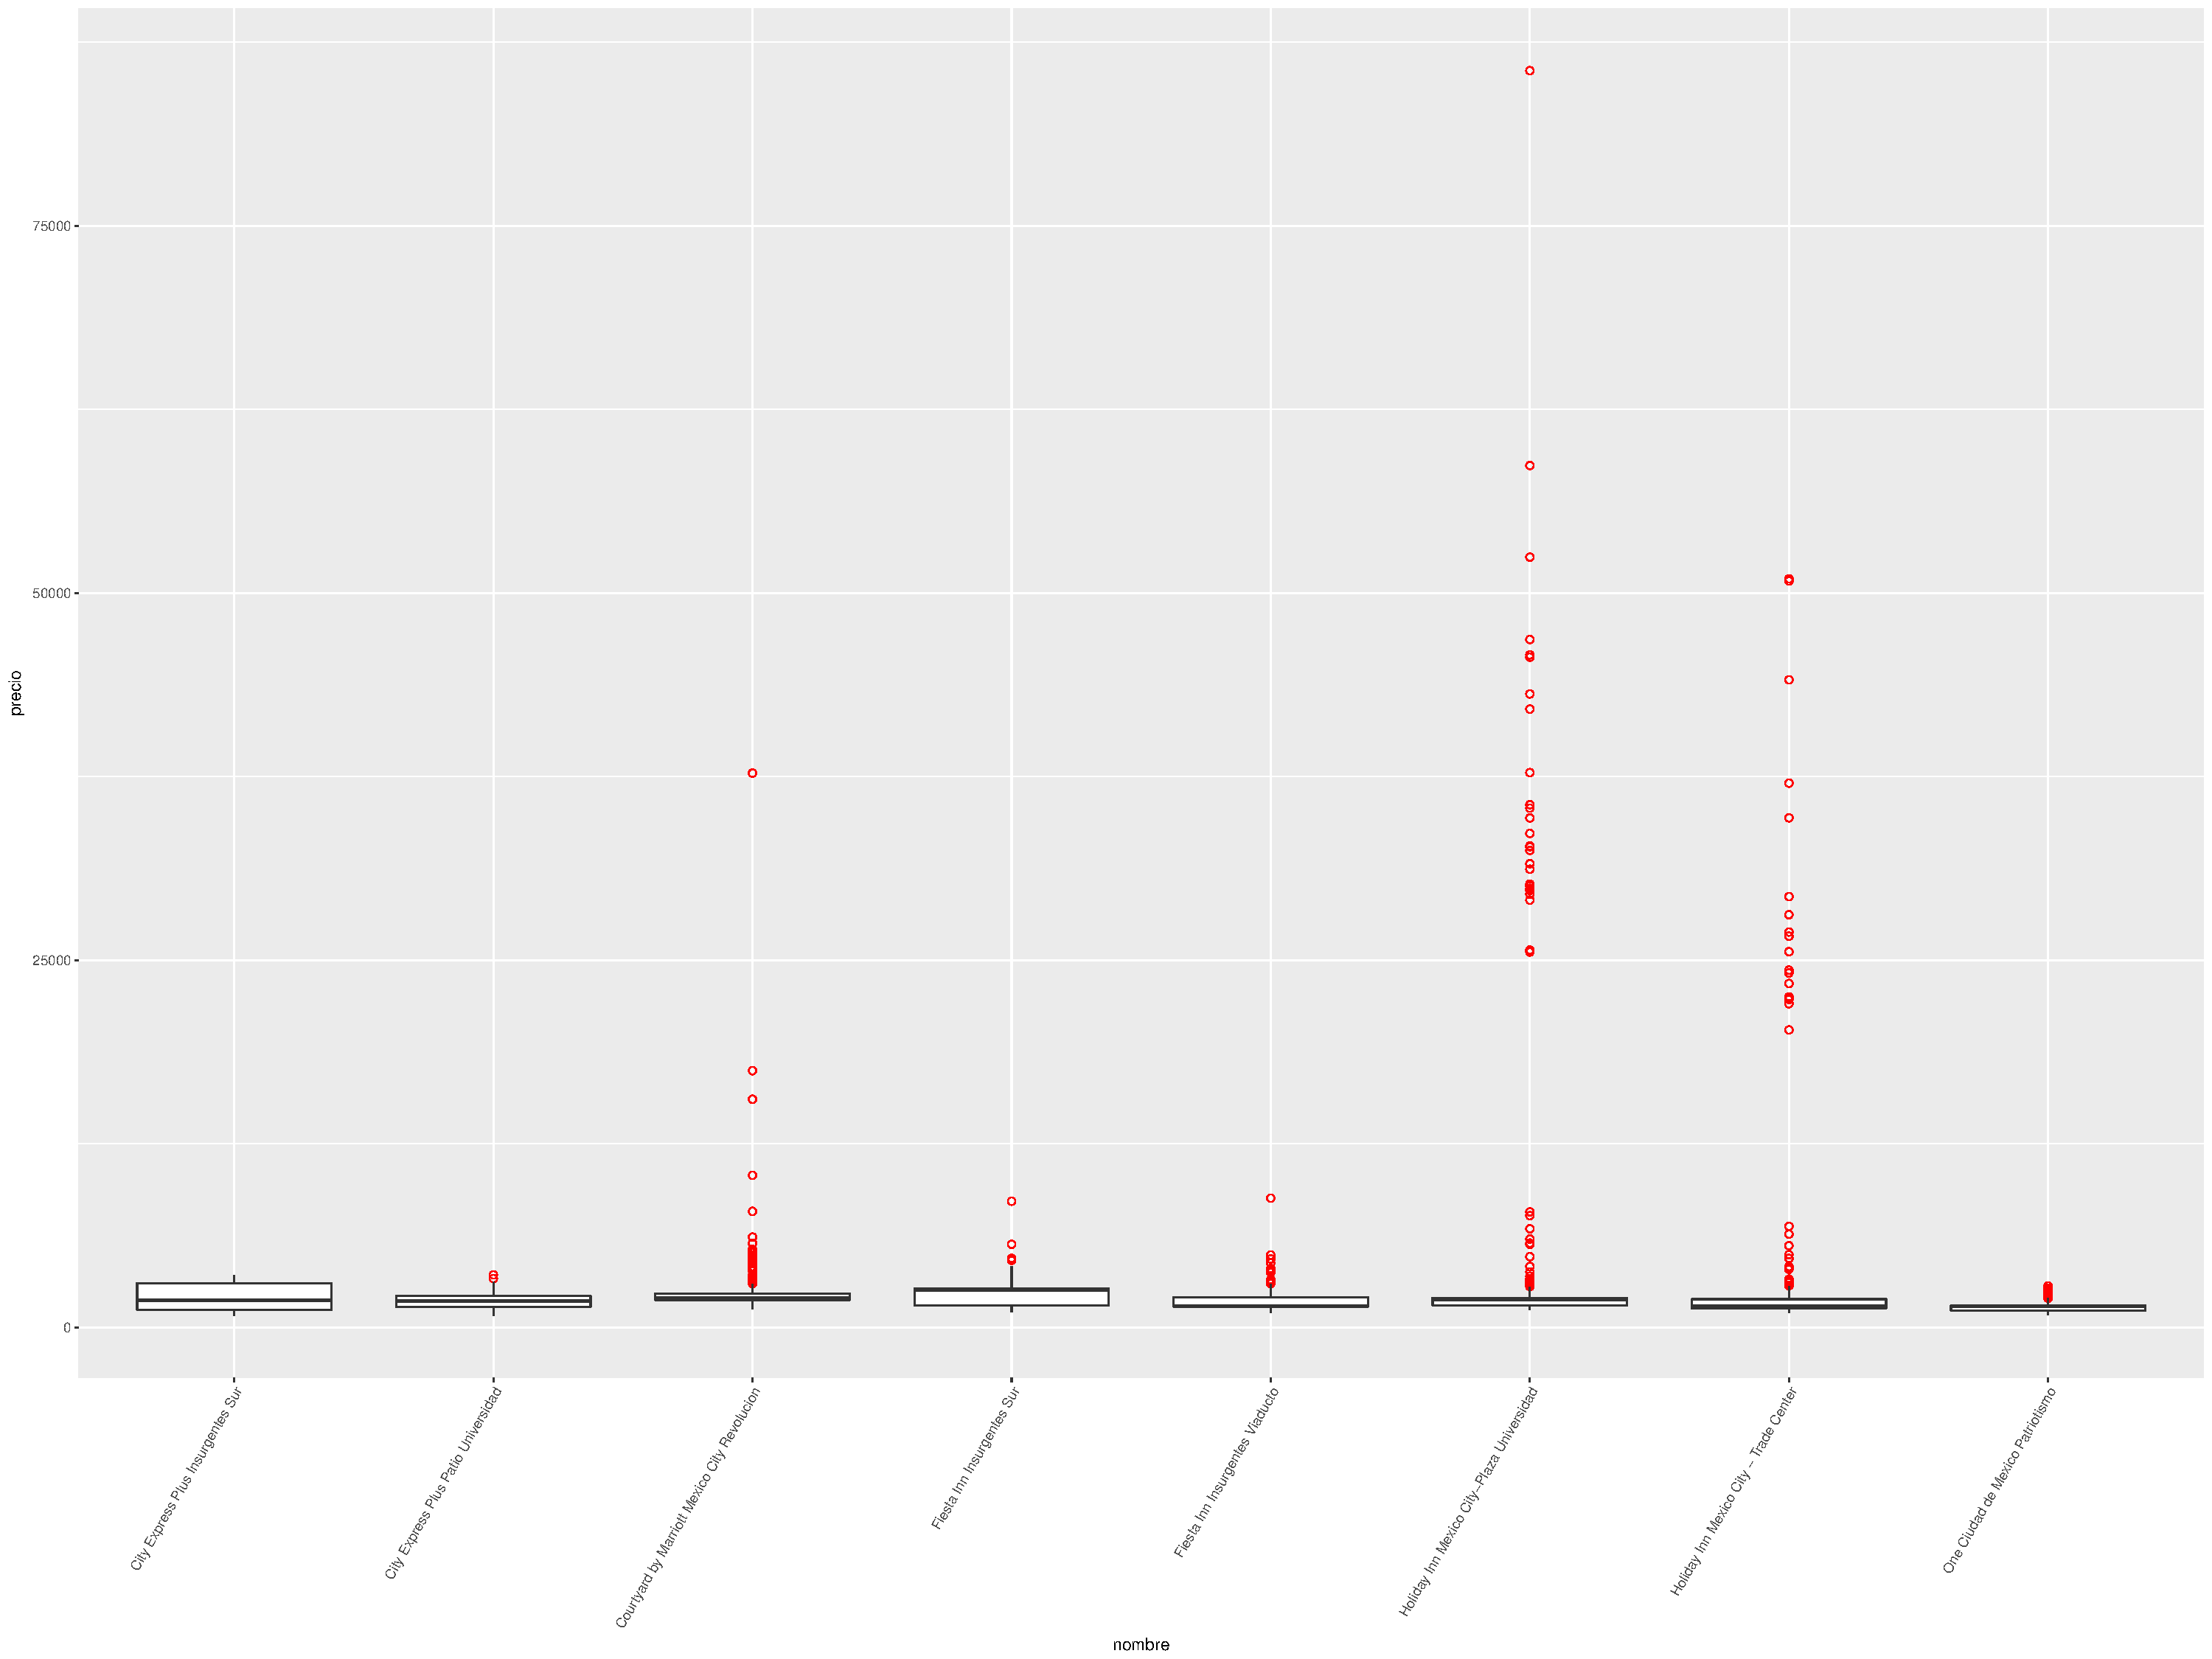
\includegraphics[width=\maxwidth,height=8cm]{figures/PreciosBoxPlot-1}    
  \caption{Precios de la competencia en el tiempo}
\end{figure}

Los datos atípicos fueron eliminados antes de proceder a trabajar con el módelo final.

En el siguiente apartado detallaremos cómo se utilizaron los datos presentados para la construcción del modelo de predicción de demanda y maximización de ingresos.


\section*{Modelo de Predicción de Demanda}

El modelo de predicción de demanda toma como entrada los datos de las curvas de \emph{pickup} para el hotel para cada día del periodo estudiado. Estas curvas describen la velocidad con la que una propiedad vende su inventario para un día en específico. El objetivo del modelo propuesto es utilizar estos datos para ajustar una curva que resuma el comportamiento de la propiedad en un día similar al estudiado y de esta forma generar una predicción de los cuartos ocupados en la propiedad y los días de antelación con los que serán vendidos.

Este modelo está compuesto por dos módulos principales. El primero es una regresión \emph{Poisson} definida como $log(E(Y|X)) = \beta_0 + \beta_1X$, que se alimentará con las curvas de \emph{pickup} que describen el comportamiento del hotel. Cómo resultado de este módulo obtendremos un parámetro $\beta_0$ y un parámetro $\beta_1$ que describen la curva que mejor ajusta al \emph{pickup} del hotel.

A continuación se muestra un resumen del conjunto de datos que alimentan al primer módulo del modelo de predicción de demanda:

\begin{table}[H]
\centering
\begin{tabular}{llll}
date\_create & date\_in   & antelacion & rooms \\
2017-03-16   & 2017-05-01 & 45         & 1     \\
2017-03-30   & 2017-05-01 & 31         & 2     \\
2017-04-02   & 2017-05-01 & 28         & 3     \\
2017-04-04   & 2017-05-01 & 26         & 4     \\
2017-04-11   & 2017-05-01 & 19         & 7     \\
2017-04-17   & 2017-05-01 & 13         & 8     \\
2017-04-18   & 2017-05-01 & 12         & 9     \\
2017-04-20   & 2017-05-01 & 10         & 10    \\
2017-04-21   & 2017-05-01 & 9          & 11    \\
2017-04-24   & 2017-05-01 & 6          & 20    \\
2017-04-25   & 2017-05-01 & 5          & 24    \\
2017-04-26   & 2017-05-01 & 4          & 28    \\
2017-04-27   & 2017-05-01 & 3          & 34    \\
2017-04-28   & 2017-05-01 & 2          & 56    \\
2017-04-29   & 2017-05-01 & 1          & 62    \\
2017-04-30   & 2017-05-01 & 0          & 71    \\
2017-05-01   & 2017-05-01 & -1         & 72    \\
\end{tabular}
\caption{Datos de entrada para el modelo de pronóstico de demanda} 
\end{table}

Una vez obtenidos los parámetros $\beta_0$ y $\beta_1$ de la regresión \emph{Poisson}, se procede a generar predictores potenciales de la demanda a partir de los datos con los que contamos para este análisis.

Los predictores definidos son:

\begin{itemize}
  \item diaSem: Definido como factores que van de Lunes a Domingo
  \item Mes: Definido como factores que van de Enero a Diciembre
  \item Eventos: Toma el valor 1 si la plaza cuenta con algun evento social, deportivo, o de entretenimiento en esa fecha, 0 en caso contrario
  \item PT: Definido como la tarifa promedio de la propiedad dividida entre la tarifa promedio de la competencia
  \item $beta_0$: El parámetro $\beta_0$ obtenido de la regresión \emph{Poisson}
  \item $beta_1$: El parámetro $\beta_1$ obtenido de la regresión \emph{Poisson}
\end{itemize}


Con estos predictores definidos se procede a alimentar una regresión lineal que calculará nuevos parámetros $\beta_{0*}$ y $\beta_{1*}$. A partir de estos nuevos parámetros se construyen las curvas de \emph{pickup} que ayuden a predecir la demanda de la propiedad en días futuros.

Una vez concluído el cálculo, se genera una matriz en la cuál se plasma la estimación del número de \emph{cuartos} ocupados que en una ventana futura:

\begin{table}[H]
\centering
\begin{tabular}{ll}
Dia        & Cuartos Ocupados \\
2018-06-01 & 92               \\
2018-06-02 & 78               \\
2018-06-03 & 96               \\
2018-06-04 & 99               \\
2018-06-05 & 132              \\
2018-06-06 & 151              \\
2018-06-07 & 138              \\
2018-06-08 & 88               \\
2018-06-09 & 77              
\end{tabular}
\caption{Pronóstico de cuartos noche ocupados} 
\end{table}

Esta matriz será la entrada del modelo que recomendará los precios por habitación para maximizar los ingresos de la propiedad.


\section*{Modelo de maximización de ingresos}

Una vez pronósticado los cuartos ocupados para cada una de las propiedades de la cadena, se alimentó un modelo de pricing dinámico que entrega recomendaciones de precios para la tarifa pública tomando en cuenta la demanda pronósticada para cierto día del año.

Típicamente el gerente de la propiedad controla la cantidad de cuartos ofrecidos a diferentes precios, es decir, se asigna cierto número de cuartos a cada nível de tarifa de tal forma que cuando el inventario asignado al precio mas bajo se agota, se consume el inventario asignado al siguiente nivel de tarifa que será mayor al primer precio ofertado.

A continuación se muestra un esquema donde se ejemplifica la idea mencionada anteriormente:

\begin{figure}[H]
  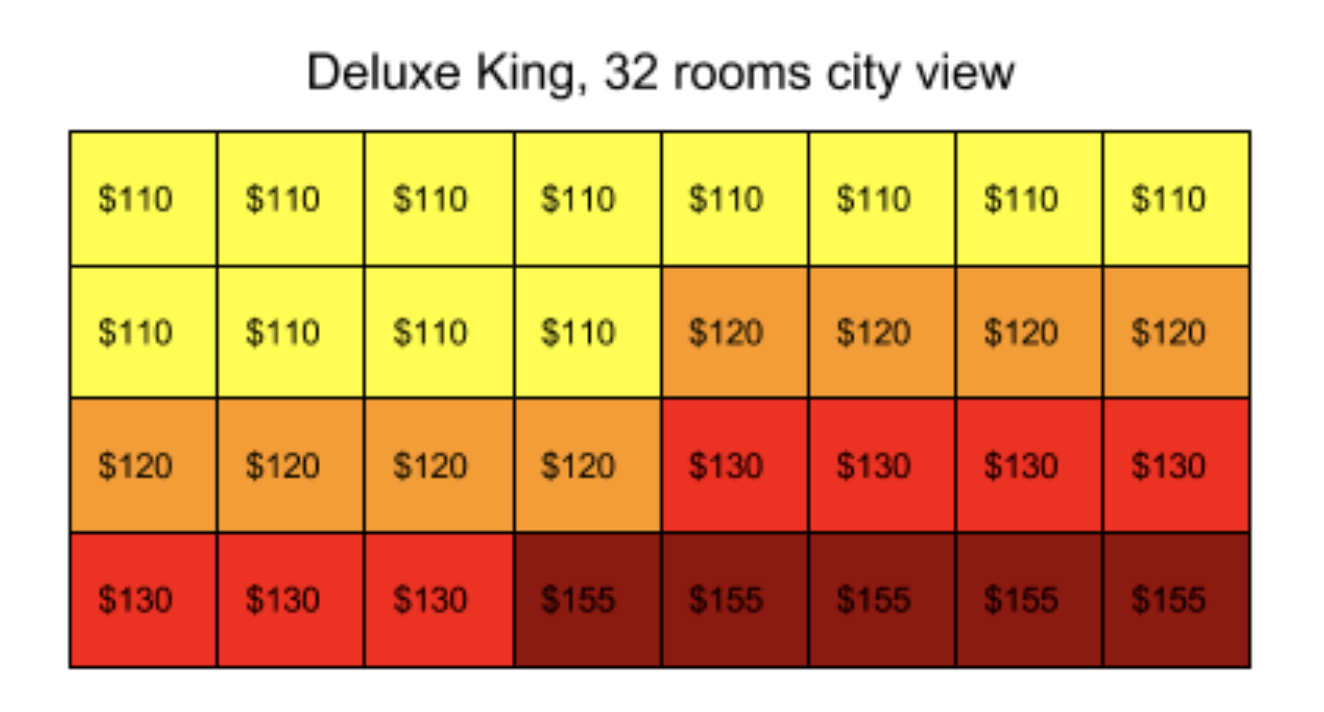
\includegraphics[width=\linewidth]{Figures/buckets.png}
  \caption{Asignacion de inventario}
  \label{fig:Asignacion de Inventario}
\end{figure}

Como se puede observar, tenemos un inventario de 32 cuartos divido en 4 níveles de precios:
\begin{itemize}[noitemsep]
\item 12 cuartos son ofrecidos a un valor de 110 USD
\item 8 cuartos son ofrecidos a un valor de 120 USD
\item 7 cuartos son ofrecidos a un valor de 130 USD
\item 5 cuartos son ofrecidos a un valor de 155 USD
\end{itemize}

\subsection*{Formulación del modelo}

Un problema de maximización de ingresos es básicamente un problema de optimización sujeto a restricciones, en este caso, se quiere maximizar la siguiente función objetivo:
$$\sum_{i=0}^{n}p_i*o_i$$
En donde i es la índice de la noche, $p_i$ es el precio del cuarto para la i-ésima noche y $o_i$ es la ocupación pronósticada (demanda) para la i-ésima noche al precio $p_i$. Asumimos también que la función de la ocupación (demanda) está sujeta al precio bajo la siguiente relación:
$$o = o_{nominal} * (\frac{p}{p_{nominal}})^e$$
Donde $o_{nominal}$ corresponde a la ocupación pronosticada para una noche dada tomando como base un precio nominal ($p_{nominal}$). Para este caso el $p_{nominal}$ es igual a la tarifa pública promediada a lo largo del año. El valor de $e$ (elasticidad) toma un valor = -2. En otras palabras, $p$ incrementa en un 10\% y la demanda decrece cerca de un 20\%.

Existen las siguientes restricciones también: $$o_i \leq Capacidad\ \forall i$$ y $$p_i > 0\ \forall i$$

En otras palabras, la ocupación no puede exceder a la capacidad del hotel y los precios deben ser siempre mayores a cero.

Una vez definidas la función objetivo y las restricciones, se ejecuta el modelo de optimización utilizando el método de \emph{Programación cuadrática secuencial}, un algóritmo útil para resolver problemas de optimización no lineales.

El método de \emph{programación cuadrática secuencial} es un método iterativo para problemas optimización no-lineales con restricciones. Este método es utilizado en problemas matemáticos en los cuáles la función objetivo y las restricciones son doblemente continuamente diferenciables.

En \emph{programación cuadrática secuencial} se resuelven una serie de subproblemas de optimización de un modelo cuadrático de la función objetivo sujeta a una linearización de las restricciones. Si el problema no cuenta con restricciones, el método se reduce al \emph{método de Newton} para encontrar un punto donde el gradiente de la función objetivo desaparece. Si el problema tiene restricciones de igualdad, el método es equivalente a aplicar el \emph{método de Newton} para encontrar las condiciones óptimas de primer orden o las condiciones de \emph{Karush-Kuhn-Tucker}

Las bases del aglorítmo son las siguientes:

Se debe considerar un problema no-lineal de la forma: $$\min_x f(x)$$ Sujeto a $$b(x) \geq 0$$ $$c(x) = 0$$

El \emph{Lagrangiano} para este problema es: $$\mathcal{L}(x,\lambda,\sigma)=f(x)-\lambda^Tb(x)-\sigma^Tc(x)$$

Donde $\lambda$ y $\sigma$ son \emph{multiplicadores lagrangianos}. En la iteración $x_k$, el aglorítmo de programación cuadratica secuencial define la dirección de búsqueda apropiada $d_k$ como solución al subproblema de programación cuadrática: 

$$\min_d f(x_k) + \nabla f(x_k)^T d + \frac{1}{2}d^T \nabla_{xx}^2 \mathcal{L} (x_k,\lambda_k,\sigma_k)d$$
Sujeto a
$$b(x_k) + \nabla b(x_k)^T d\geq 0$$
$$c(x_k) + \nabla c(x_k)^T d = 0$$

Para fines de este trabajo de investigación, se utilizó la implementación del método \emph{SQP} contenido en el paquete \emph{Scipy} en  \emph{Python}

Para poder hacer una asignación dinámica de los precios, evitando tener que correr el modelo conforme la información del hotel es actualizada, se partió el inventario en 4 níveles de disponiblidad (159,120,80 y 40 cuartos disponibles). Para cada nível de capacidad se resolvió la función objetivo para obtener 4 conjuntos de precios, de esta forma, el gerente de la propiedad puede saber a qué nível de precio debe subir la tarifa pública de la propiedad conforme las habitaciones disponibles decrecen.

El modelo de maximización de ingresos arroja como resultado una matriz de día vs precio por niveles de inventario. A continuación se muestra un ejemplo:
\\
\\

\begin{table}[H]
  \centering
  \csvautotabular{data/rates.csv}\par
  \caption{Matriz de asignacion de precio por inventario disponible} 
\end{table}

De la matriz que arroja el modelo de optimización de precios podemos obtener el precio sugerido para cada nivel de inventario disponible por día pronósticado. Por ejemplo, para el día 7 de julio de 2018 el modelo sugiere un precio público para habitación sencilla de \$784.76 si el hotel tiene entre 121 y 159 habitaciones disponibles; \$903.32 si se tienen entre 81 y 120 habitaciones disponibles; \$1106.34 enre 41 y 80 habitaciones disponibles; y finalmente un precio de \$1476.07 entre 1 y 40 habitaciones disponibles.

\subsection*{Consideraciones del modelo}

Este modelo se formuló considerando los siguientes puntos:
\begin{itemize}[noitemsep]
  \item Se consideran estancias de una sola noche
  \item No se toman en cuenta reservaciones para grupos ni cancelaciones
  \item Asusmimos paridad de precios entre los canales, es decir, los precios no varían entre los canales de venta
  \item Se considera solamente un tipo de habitación, el incremento por cambio de habitación es un monto fijo conocido como gap
  \item Se asume un valor para la elasticidad (-2) que es un valor razonable para la industria
\end{itemize}

En el siguiente capítulo se discutirá acerca de la interpretación del modelo propuesto y los resultados obtenidos.
